% Project Specifications
\clearpage%if the chapter heading starts close to bottom of the page, force a line break and remove the vertical vspace
\vspace{21.5pt}
\chapter{Project Specifications/Background}

To perform the needed recovery operations as described in the previous section the project has to be able to perform several operations.

Both standard Raspberry Pi Pico and Raspberry Pi Pico W are likely to be used, so the project should be able to support both and automatically detect the attached target type.

These images have to be stored  on the recovery board, and a method to update the images.

Preferably this updating would be handled by the recovery board itself, without using some form of accompanying image rebuilder on a computer, in order to keep platform independence and simplicity of operation.

The project should be able to interface with a target board to query file system status and perform file system operations to recover target board from potential non booting status, including zeroing out full file system to perform a quick reset, or reimage a full firmware to target board.

This project is specified to be done using a Raspberry Pi Pico operating standalone without a computer for convenience to use existing resources, and as a potential demonstration of a use for a Pi Pico.

\clearpage
\section{Hardware}

\subsection{Overview of Raspberry Pi Pico}

\begin{figure}[ht]
	\centering
	\AltText{Stock photo of Raspberry Pi Pico}{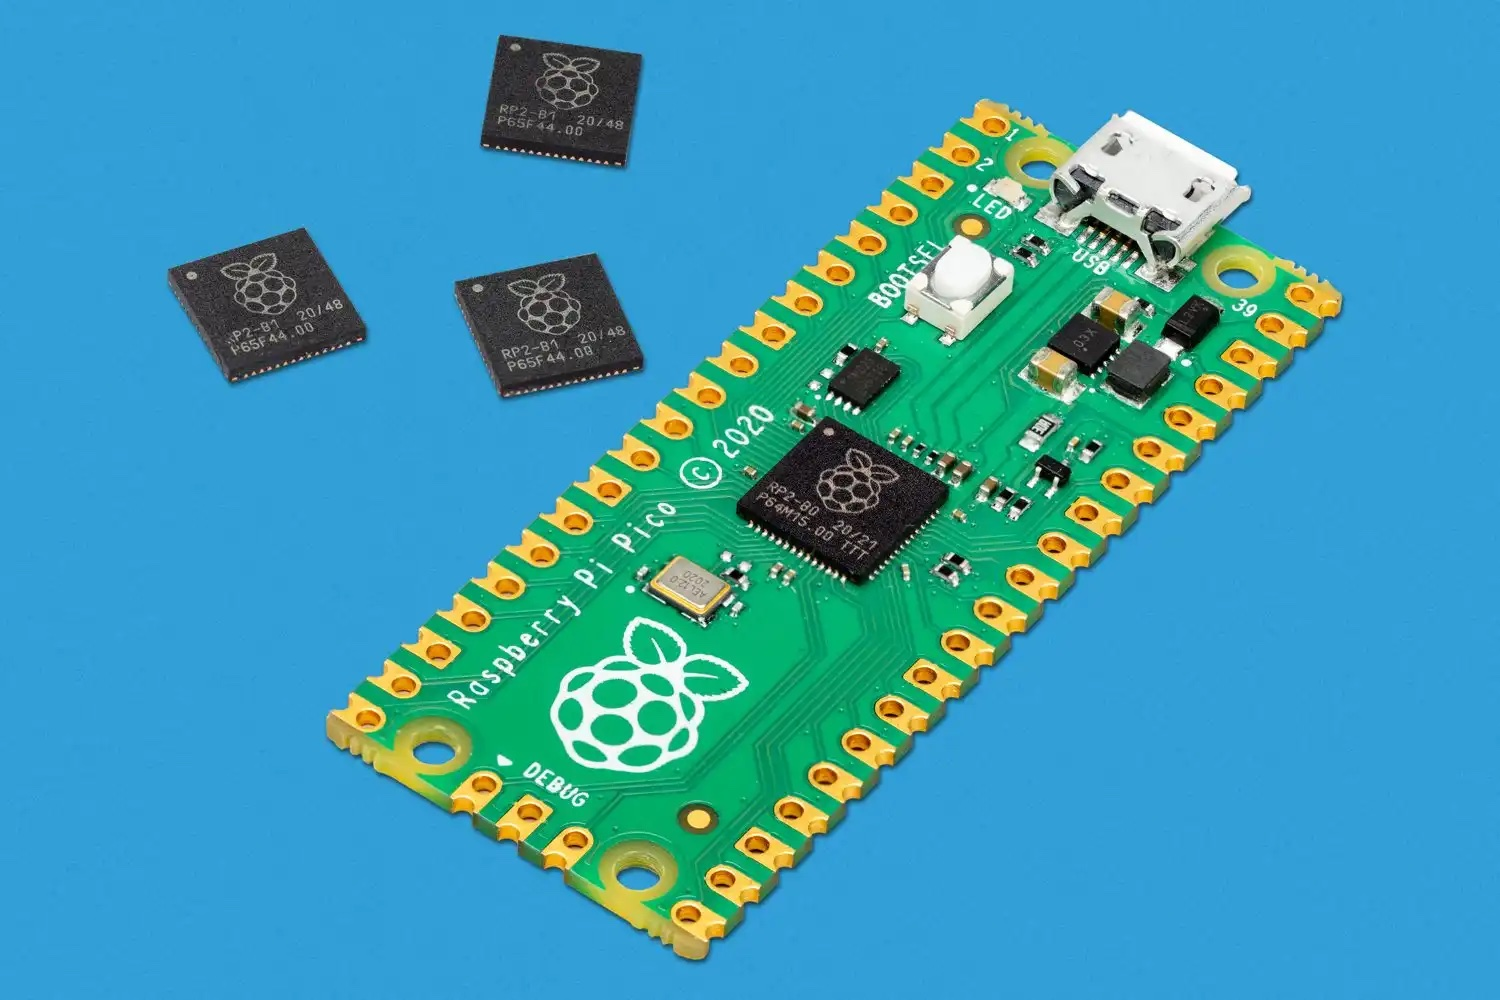
\includegraphics[width=\textwidth]{pico-rp2040}}
	\caption{Stock photo of Raspberry Pi Pico\cite{ltdBuyRaspberryPi}}
	\label{fig:picostock}
\end{figure}

The principle target recovery baord and project board are both a Raspberry Pi Pico.

The Raspberry Pi Pico \autoref{fig:picostock} is a compact \gls{mcu} development platform created by the Raspberry pi foundation, running a dual core \gls{arm} Cortex M0 at 133Mhz with a larger than typical 264kB inbuilt \gls{ram} and 2MB of \gls{spi} flash memory storage for the class of \gls{mcu}\cite{ltdBuyRaspberryPi}.

The Pico is capable of having software programmed to it via inbuilt ROM USB flasher using a UF2 image or via \gls{swd} interface.

\subsection{Pico Display Pack}
A Pimoroni Pico DIsplay Pack\autoref{fig:picodisplaypack} was selected as the user interface hardware for development due to availability on hand, but is a non critical component that could be swapped for other displays and input with relatively minor adjustment.

The Display Pack features four tactile buttons and a 1.14” 240x135 pixel IPS LCD screen to allow user feedback and input.

\begin{figure}[ht]
	\centering
	\AltText{Stock photo of Pimoroni Pico DIsplay Pack}{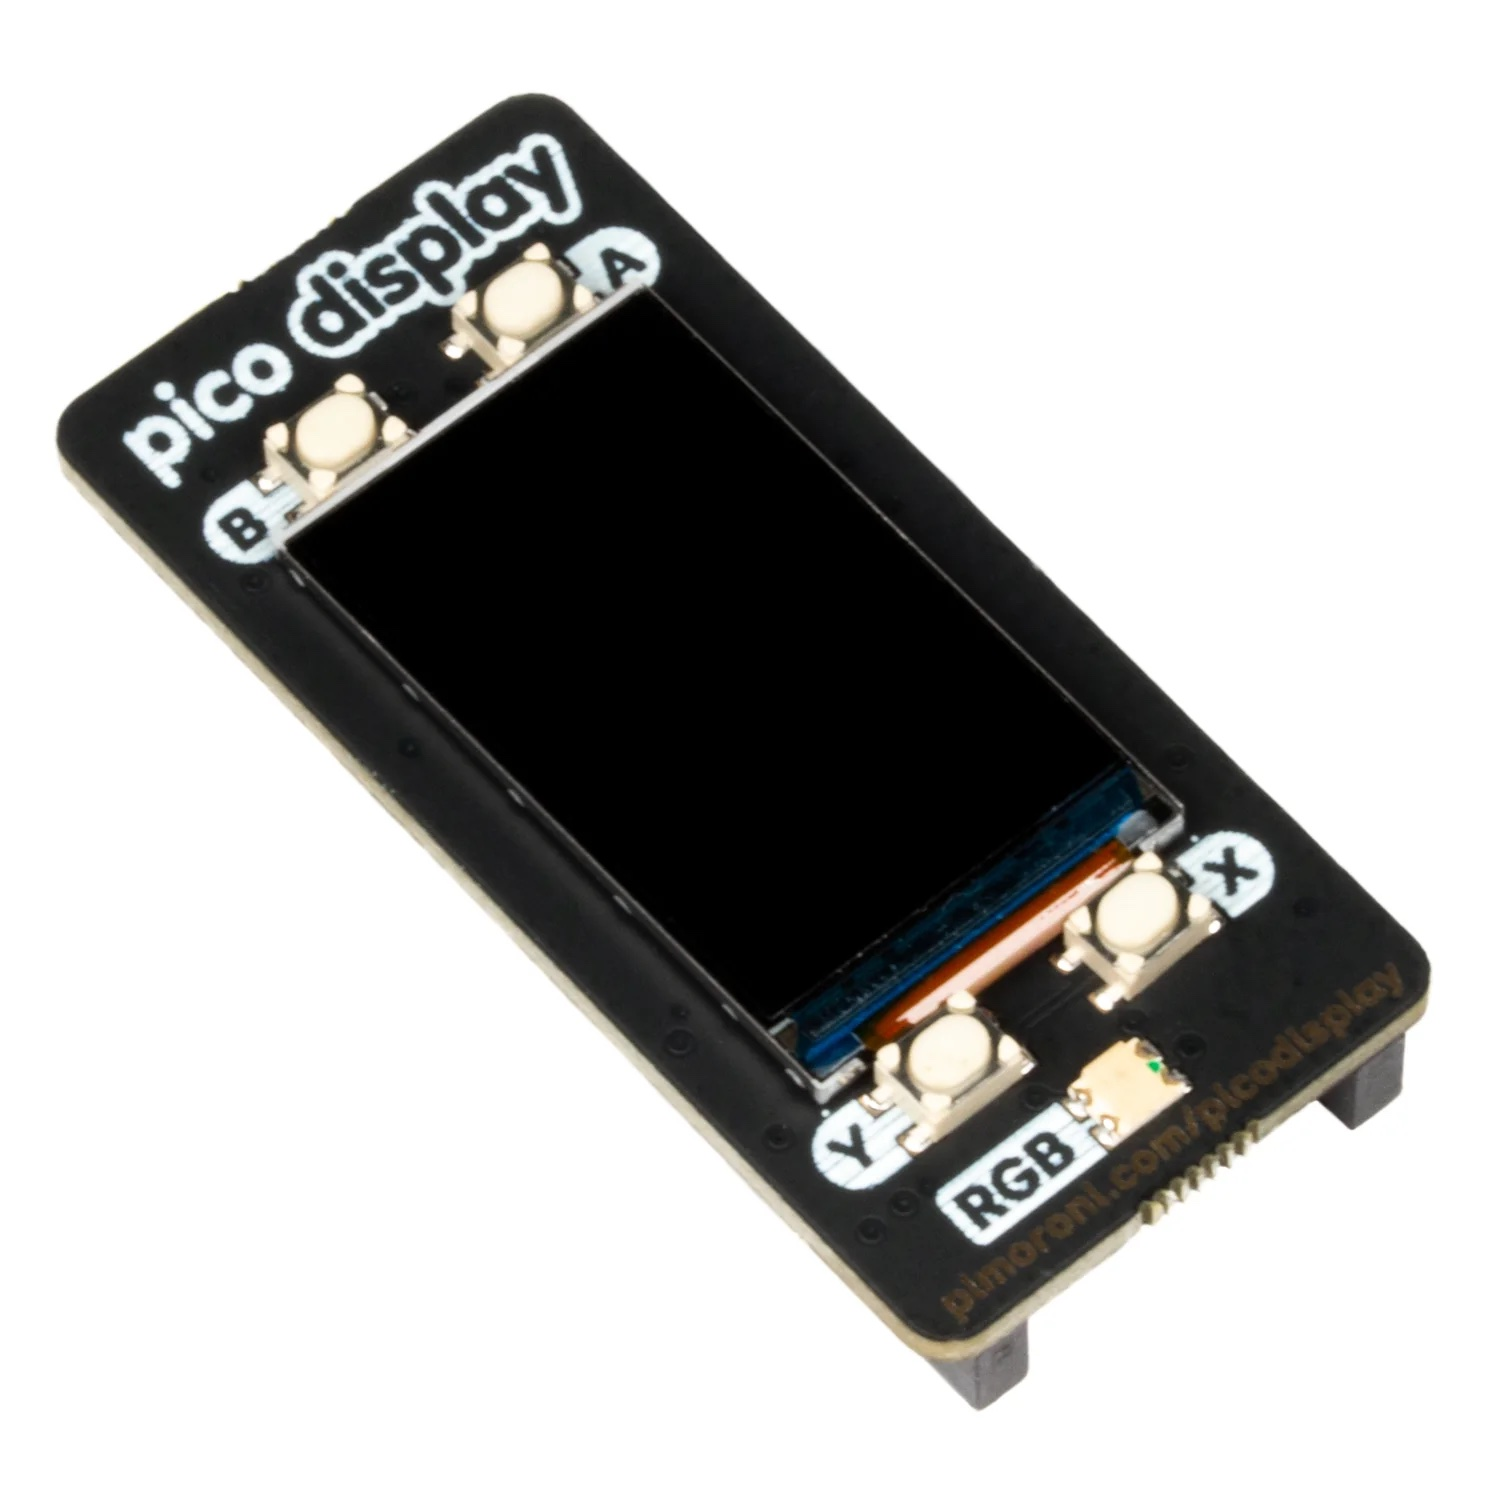
\includegraphics[width=.66\textwidth]{picodisplaypack}}
	\caption{Stock photo of Pimoroni Pico DIsplay Pack\cite{PicoDisplayPack}}
	\label{fig:picodisplaypack}
\end{figure}
	
\clearpage
\subsection{J-Link EDU Mini}
For debugging and rapid prototyping a J-Link EDU Mini\cite{JLinkEDUMini}\autoref{fig:jlinkedumini} was used as the hardware debugger for project to enable.

This is a \gls{usb} compact hardware debugger for embedded platforms to provide direct flashing and debug access to the Pi Pico to provide a more convenient development environment with one click compiling and target flashing.

\begin{figure}[ht]
	\centering
	\AltText{Stock photo of J-Link EDU Mini}{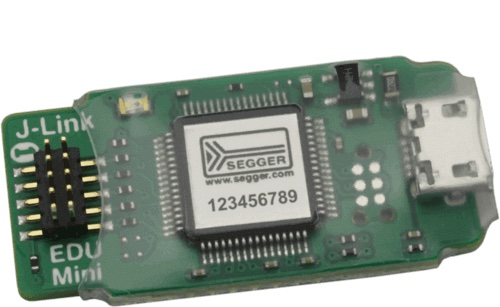
\includegraphics[width=.66\textwidth]{jlinkedumini}}
	\caption{Stock photo of J-Link EDU mini\cite{JLinkEDUMini}}
	\label{fig:jlinkedumini}
\end{figure}

\clearpage
\section{Ways to access raspberry pi pico flash}

There are a couple of potential ways to be able to access the flash memory on the pico to be able to alter or reflash it as desired.

The most common and usually used method is by holding down the 'BOOTSEL' button when plugging the pi into \gls{usb}, which disabled the \gls{spi} flash memory chip select line temporarily during boot process and causes the \gls{mcu} to automatically go into flashing mode whereupon the chip presents a virtual fat drive as a mass storage device to the \gls{usb} host allowing an image to be dragged on and flashed.

This method could be used to run a \gls{ram} resident program via specific UF2 loading addresses which could be used to examine the flash memory and run an automatic recovery of a filesystem from MicroPython without affecting the primary flashed application.

But this method is cumbersome, as it cannot be fully automated due to the requirement of manual BOOTSEL enablement to enable whilst plugging in. There are ways to enter recovery mode without pressing BOOTSEL via \gls{usb} interface using picotool application that can make negotiate a pico running firmwares based on standard \gls{usb} stack to reboot into recovery mode\cite{picotool}, but this is inflexible and would not help recovering an application that immediately disables USB automatically at boot which is one of the primary requirements of the project.

The other principle method of being able to arbitrarily access flash memory on pico is via the \gls{arm} \gls{swd} debug interface using the board accessible debug pads intended for direct programming and onchip debugging\cite{ARMDebugInterface}.

The \gls{swd} interface  is always available regardless of firmware setup, and allows full control of the chip thus making it possible to fully automate. The principle disadvantage of this approach is the less convenient physical access to the interface compared to connecting to a \gls{usb} host.
\clearpage
\section{SWD interface}
The \gls{arm} \gls{swd} interface is an \gls{arm} microdevices created standard for all \gls{arm} Cortex CPU's using two wires for clock and signal, that allows bidirectional communication over a single signal wire and a variable host controlled signal speed.

Typical \gls{swd} control speeds range from 4-25MHZ clock, though to achieve high clock rates typically seperate hardware such an \gls{fpga} programmed for dedicated signal control is used. Bue due to the debugger controlled clock, timing is not critical and can be flexible allowing a more simplistic 'bit banging' approach to be used from any GPIO interface, though more refined methods utilising peripheral hardware inside an \gls{mcu} can be possible, such as \gls{spi} controller, or in the case of the pi pico it has a programmable io interface that can be utilised for \gls{swd} as utilised in the pi foundations pi pico based debug probe. un

Communication with the debug unit is first established with a reset sequence, which will always reset the debug unit to a known starting state so that connection can be established regardless of existing state.

Every transaction consists of a multiple phase process. First a request header to signal read or write a register including contained command validation parity check is clocked out onto the \gls{swd} I/O line, after which the host switches to reading the I/O line and clocks in three bytes to check for an acknowledgement reply indicating whether the request was received, debug unit is busy or can action the request, or if the debug unit is in fault state.

If the acknowledgement is an all OK, then the next action is either clocking in the bus for length of data to read response, or switching back to clocking out the  transmitted data packet.

In the case of \gls{ap} memory reads, the first read after a read request has to be ignored and discarded to give the debug unit time to retrieve the memory data, thus read cycle will always have an extra throwaway read at the end also.

After a data transfer if no other command is to be immediately processed an extra 8 clock cycle idle has to be continued post transfer to allow the debug unit to process.

\begin{figure}[ht]
	\centering
	\AltText{Diagram of ARM SWD memory write operation}{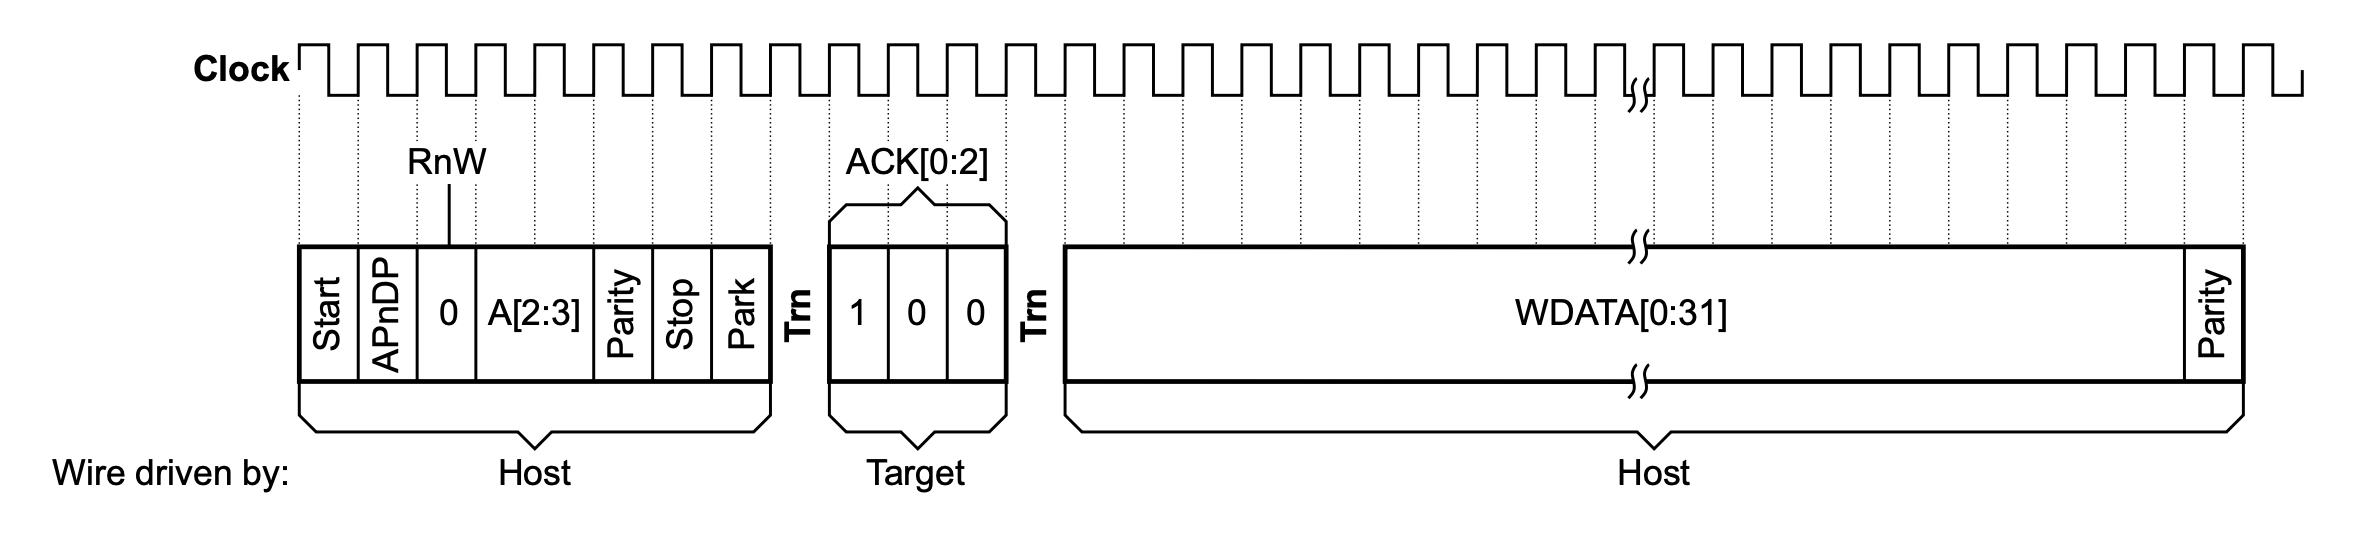
\includegraphics[width=\textwidth]{armswdwrite}}
	\caption{Diagram of SWD memory write\cite{ARMDebugInterface}}
	\label{fig:armswdwrite}
\end{figure}
\clearpage

\gls{arm} \gls{mcu}'s can also optionally support \gls{jtag} protocol debugging, using the same pins as \gls{swd}. For chips supporting both a handshake to establish the protocol being used is needed. But as the pico is an \gls{swd} only \gls{mcu}, this part of the connection protocol is not needed.

Each CPU core has it's own debug unit, along with a third 'reset' unit that can be used to reset the whole \gls{mcu}

\gls{swd}  control allows commanding a debug unit in the \gls{mcu}, which can read and write memory, control execution. set breakpoints and other debug aiding measures.

\gls{swd} itself cannot directly access the flash memory on the pico, to do this the \gls{mcu} has to be instructed via memory access and process control to perform the accesses required.

This can be done two different ways, direct instructions to perform requires actions can be written into memory
boforehand and jump to execute step by step direct flash programming, though this would be very inefficient due to amount of waiting for writes to complete.

A simpler and more reliable method typically used for flash programming via debuggers is uploading a small stub flash loader application which which the debugger communicates via a defined shared memory space, where some form of flashing cache buffer can be filled for the stub to continue programming.

For controlling the \gls{swd} interface there are multiple possible methods to consider. 

So called 'bit banging' \gls{gpio} signals utilising \gls{arm} code to control signal lines via direct access which is effectively entirely non hardware dependant.

Using a programmable I/O module in the Pico which allows a lower level clock accurate control of \gls{gpio} on the device, an example implementation of which available in the official Raspberry Pi Pico debugger PicoProbe project\cite{Picoprobe2023}.

It is also potentially possible to utilise \gls{spi} peripheral in order to perform \gls{swd} transactions, though this was deemed unnecessarily complicated to investigate as a potential solution\cite{OpenOCDRaspberryPi}.

Due to \gls{swd}'s use of host device clock signal and no tight requirements for it's running, the simpler 'bit banging' was implemented as first proof of concept, setting the pico clock
\clearpage
\section{UF2 file format}
UF2 is a file format created by Microsoft with the intention of having a simple universal file format for device firmware image updates, that is very easy to support with a minimal loader to manage the flashing on target device, including frequently via a \gls{usb} mass storage supporting bootloader that presents a virtual file system to the operating system via standard \gls{usb} mass storage protocol, so that special hardware and software is not needed for firmware updates.

A Uf2 file is made up of 512byte blocks, each of which has a header specifying the blocks address in \gls{rom}, typically a family code to indicate what device the image is meant for, the relative number of specific 512byte block, and a total block count. 

UF2 contains a flag field to allow optional features in the format, including a checksum for the data and presence of family type instead of file size which is typically used instead of the defauly file size field, owing to this size data being calculable from the stored block data. Checksum data is not typically used, and thus not needed to be implemented.

This is enough information for flashing software to know where to put each part of image as received, and keep track of progress in order to know full image has been received without an explicit end of transfer, which is key to being able to flash images via \gls{usb} mass storage filesystem write.

The format was chosen by the pi foundation as the native image format for the pico due to this simplicity of use, and the pico recovery bootloader presents a \gls{usb} mass storage virtual \gls{fat} file system from it's \gls{rom} stored 16kB alongside \gls{usb} stack and \gls{rom} callable routines for functionality including \gls{spi} flashrom writing.

The inbuilt bootloader uses the target address of the image to signify whether to load the data into ram for immiediete execution, or to flash and execute from \gls{spi}.

\clearpage
\section{USB Virtual Filesystem}
Standalone \gls{swd} control is enough to be able to recover a file system or erase a board to rescue bootloader state, but in order to fully setup a pico from scratch a flash image to program is needed. This image could be included into the program as a binary include, but this makes updating cumbersome requiring recompiling and uploading a new full binary image to the recovery pico.

This is typically achieved by setting the pico into BOOTSEL recovery mode and flashing the new combined uf2 image on.

It was figured that a more convenient alternative would be for the device to manage it's own images, which also allows device to signal what firmware is installed to the user via filename.

The project has to support pico original and w editions, so two firmwares need to be stored.

The UF2 format was created for simplicity of flashing to hardware via a bootloader, and is quite wasteful internally, each 256B block of target flash uses a full 512B in the file to make addressing simple, which leads the file to be nearly half empty due to header data for the 256B blocks only occupying a small portion of the remaining 256B.

This header data is mostly static, barring changing addressing data, thus it is possible to generate this data using only a list of addresses per block. This allows the possibility to generate a custom storage format to save storage and allow a standard 2MB pico enough storage to save flash images for typical use cases for both models.

All the UF2 header data barring addresses can be calculated at run time, so only the addresses for each flash block are required to be stored in a header, empty flash does not waste image space, nor non payload areas of the original uf2 image, thus virtually

\clearpage
\section{MicroPython Filesystem}
One of the primary goals of the project is to recover a non booting MicroPython installation on a pico, this requires interfacing with the local file system in some way.

MicroPython as a project supports various different file systems such as FAT, but for the pi pico port the filesystem used is the open source littlefs filesystem\cite{MicroPythonProject2023}.

The littlefs file system is designed specifically for \gls{mcu}'s, designed to be safe for use in environments where constant power is not guaranteed and data integrity is needed by using a copy on write methodology where all updates to files are performed on a dynamic copy of the data with file table only updated when commit is complete and file closed to allow automatic fallback to last good state on unexpected power loss.





